% ============================================================
% APPENDIX A — MATHEMATICAL DERIVATIONS
% ============================================================
\chapter{Mathematical Derivations}
\label{app:derivations}

Derivations for the physical models and signal-processing justifications used in the main text.

\section{Curvature Drop}
\label{sec:curv_derivation}

Over a spherical Earth of radius $R_E$, an observer at height $h_o$ sees a horizon at distance $d$. From the right triangle formed by the Earth centre, the observer, and the tangent point:
\begin{equation}
(R_E + h_o)^2 = R_E^2 + d_{\mathrm{horizon}}^2.
\end{equation}
\noindent Expanding and neglecting $h_o^2 \ll R_E h_o$:
\begin{equation}
d_{\mathrm{horizon}} \approx \sqrt{2 R_E h_o}.
\end{equation}
\noindent A terrain feature at distance $d$ appears lower because the reference horizontal curves downward by:
\begin{equation}
\delta(d) = \frac{d^2}{2R_E}.
\end{equation}
\noindent Standard atmospheric refraction effectively increases visible range. Replacing $R_E$ with $R_E / (1 - k)$ where $k \approx 0.13$:
\begin{equation}
h(d) = \frac{d^2(1 - k)}{2 R_E}, \qquad k = 0.13.
\end{equation}

\paragraph{Worked example.}
With $R_E = 6371$\,km, $k = 0.13$:

\begin{center}
\begin{tabular}{cc}
\toprule
Distance $d$ (km) & Hidden height $h$ (m) \\
\midrule
10 & 49 \\
20 & 196 \\
30 & 441 \\
40 & 785 \\
50 & 1{,}226 \\
\bottomrule
\end{tabular}
\end{center}

\noindent At 30\,km, any ridge below $\sim 440$\,m above the observer's eye level is hidden. This justifies the 30\,km ray-trace limit.

\section{Koschmieder Visibility Law}
\label{sec:koschmieder_derivation}

The Koschmieder law relates apparent contrast $C(d)$ of an object at distance $d$ to its inherent contrast $C_0$:
\begin{equation}
C(d) = C_0 \, \exp(-\sigma_{\mathrm{ext}} \, d),
\end{equation}
\noindent where $\sigma_{\mathrm{ext}}$ is the volume extinction coefficient. The meteorological visibility $V$ is the distance at which contrast drops to 2\%:
\begin{equation}
V = \frac{\ln(1/0.02)}{\sigma_{\mathrm{ext}}} = \frac{3.912}{\sigma_{\mathrm{ext}}}.
\end{equation}
\noindent Substituting:
\begin{equation}
C(d) = C_0 \, \exp\!\left(-\frac{3.912 \, d}{V}\right).
\end{equation}

\paragraph{Contrast table for $V = 50$\,km (clear mountain air).}

\begin{center}
\begin{tabular}{cc}
\toprule
Distance $d$ (km) & Relative contrast $C/C_0$ (\%) \\
\midrule
% 5 & 68.2 \\
10 & 46.5 \\
% 15 & 31.7 \\
20 & 21.6 \\
% 25 & 14.7 \\
30 & 10.0 \\
40 & 4.7 \\
50 & 2.2 \\
\bottomrule
\end{tabular}
\end{center}

\noindent At 30\,km, contrast has fallen to 10\%. This reinforces the 30\,km limit: terrain features beyond this range contribute unreliable skyline information.

\section{Cross-Correlation via FFT}
\label{sec:fft_derivation}

The Pearson normalised cross-correlation between two zero-mean signals $f$ and $g$ of length $N$ at lag $\tau$ is:
\begin{equation}
r(\tau) = \frac{\sum_{i=0}^{N-1} f(i) \, g((i + \tau) \bmod N)}{\sqrt{\sum_i f(i)^2 \cdot \sum_i g(i)^2}}.
\end{equation}

\noindent The numerator is a circular cross-correlation. By the correlation theorem:
\begin{equation}
(f \star g)[\tau] = \mathrm{IFFT}\!\big(\mathrm{FFT}(f) \odot \overline{\mathrm{FFT}(g)}\big)[\tau],
\end{equation}
\noindent where $\star$ denotes circular cross-correlation, $\odot$ is element-wise multiplication, and $\overline{(\cdot)}$ is complex conjugation. This reduces computation from $O(N^2)$ to $O(N \log N)$.

% ============================================================
% APPENDIX B — COST ESTIMATE
% ============================================================
\chapter{Cost Estimate}
\label{app:budget}

The project was developed entirely using open-source software and publicly available data. No hardware was purchased. Table~\ref{tab:budget} itemises the costs incurred.

\begin{table}[H]
\centering
\small
\caption{Project cost breakdown.}
\label{tab:budget}
\begin{tabular}{p{6cm}cc}
\toprule
\textbf{Item} & \textbf{Cost (NPR)} & \textbf{Remarks} \\
\midrule
Copernicus GLO-30 DEM data & 0 & Open access \\
PyTorch, ONNX Runtime, Horayzon, PyRender & 0 & Open source \\
Python, Git, VS Code & 0 & Open source \\
Kivy mobile framework & 0 & Open source \\
Google Street View imagery (evaluation) & 0 & Public \\
Personal laptop (development) & 0 & Existing \\
Google Colab (GPU training) & 0 & Free tier \\
Report printing and binding & $\sim$2000 & Department requirement \\
\midrule
\textbf{Total} & $\sim$2000 & \\
\bottomrule
\end{tabular}
\end{table}


% ============================================================
% APPENDIX C — PROJECT TIMELINE
% ============================================================
\chapter{Project Timeline}
\label{app:timeline}

\begin{figure}[H]
    \centering
    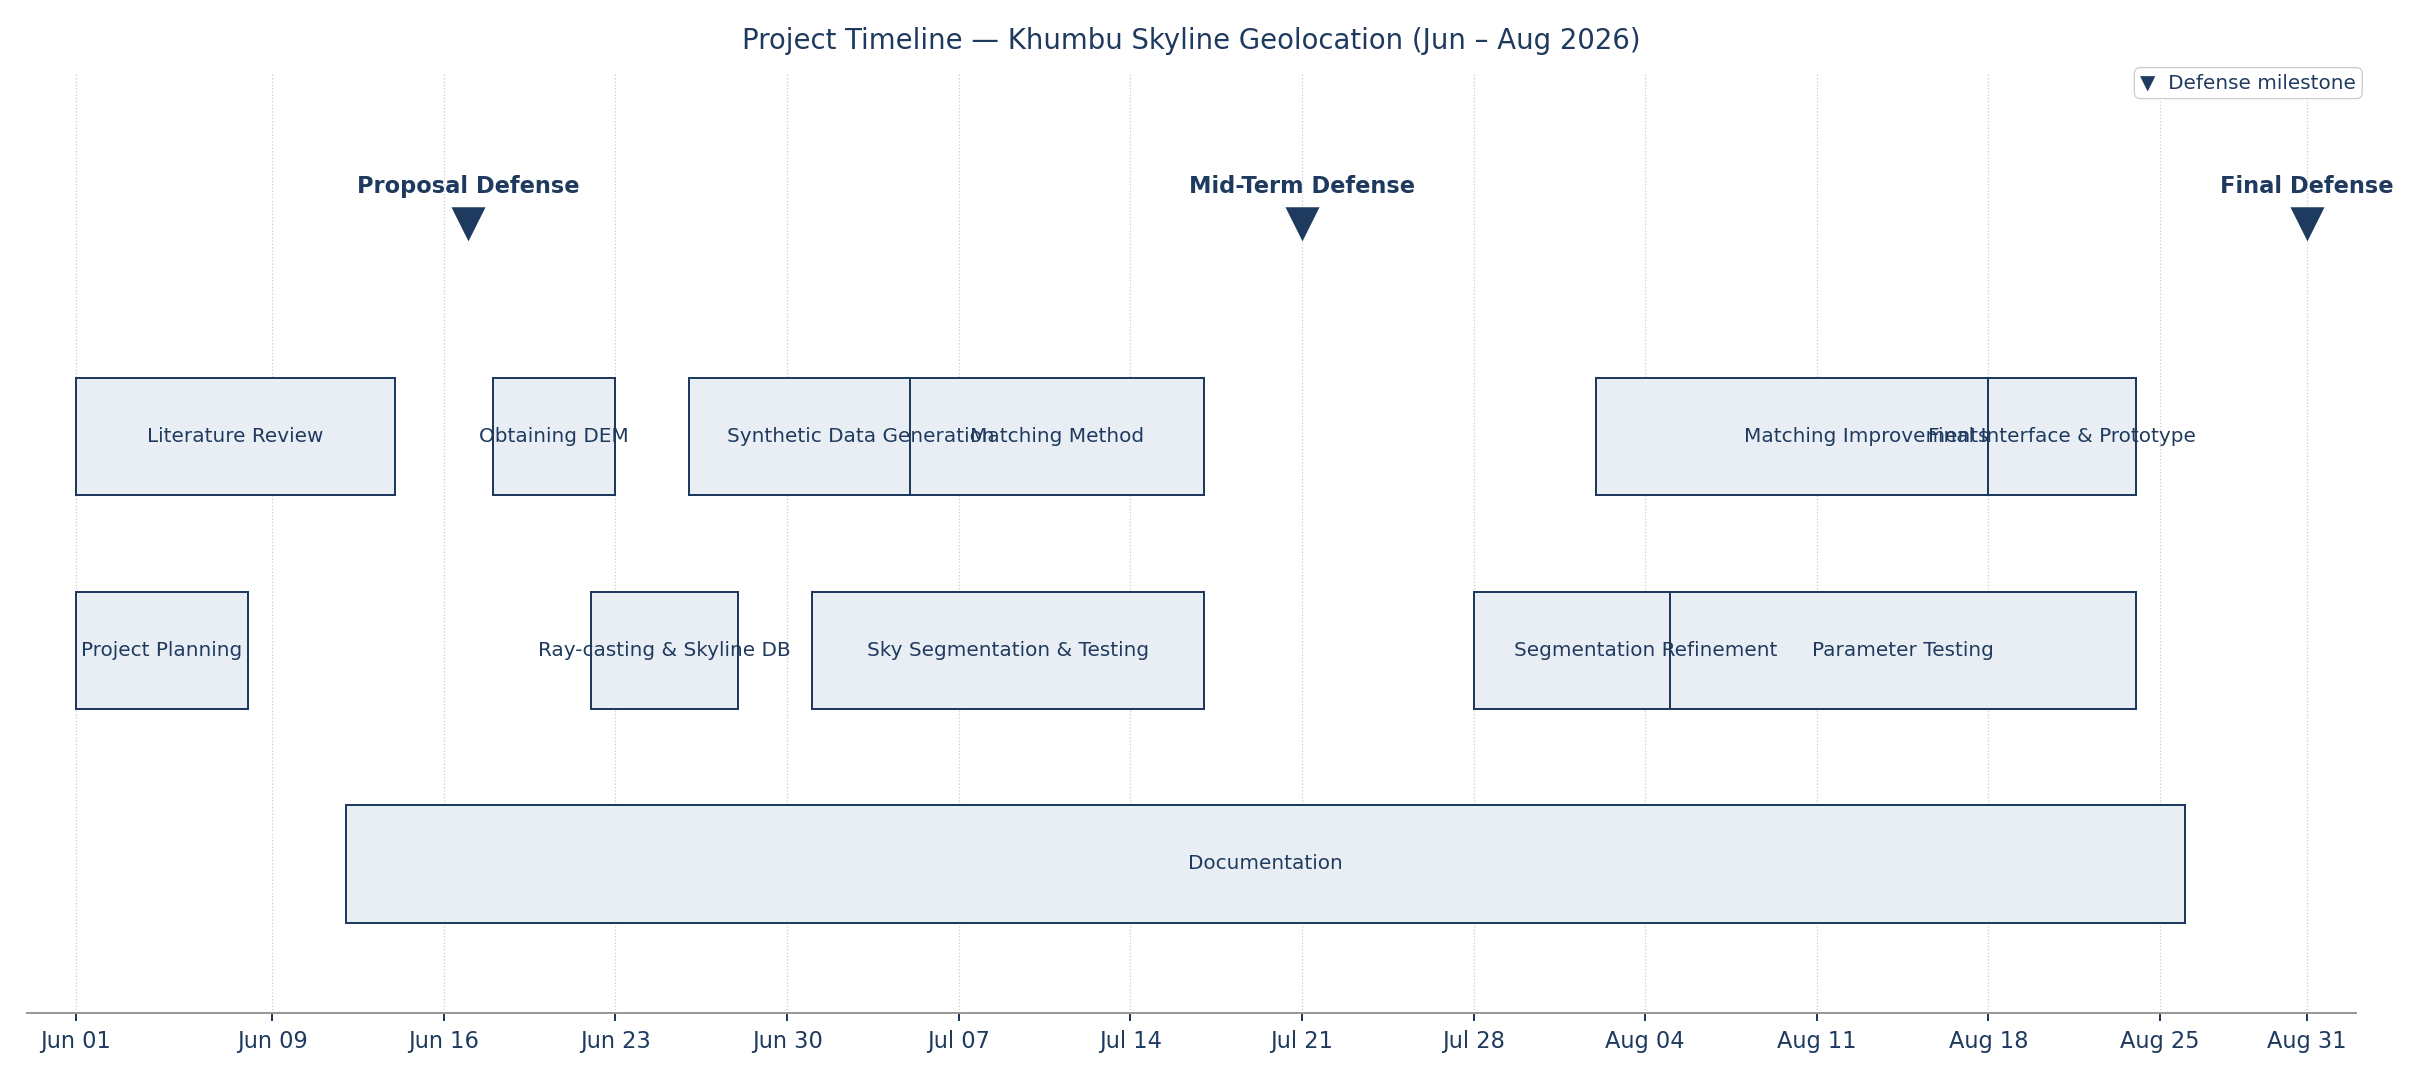
\includegraphics[width=\textwidth,height=0.68\textheight,keepaspectratio]{src/images/figures/gantt.png}
    \caption{Project Timeline.}
    \label{fig:gantt_chart}
\end{figure}


% ============================================================
% APPENDIX D — PIPELINE DIAGRAMS
% ============================================================
\chapter{Pipeline Diagrams}
\label{app:diagrams}

\section{Sky Mask Post-Processing}

\begin{figure}[H]
\centering
\begin{adjustbox}{max totalsize={0.65\textwidth}{0.85\textheight},center}
\includegraphics{src/images/postprocessing.pdf}
\end{adjustbox}
\caption{Post-processing pipeline: threshold, filter, dehaze, detect edges, fit sub-pixel, smooth.}
\label{fig:postprocessing}
\end{figure}

\section{Matching Pipeline}

\begin{figure}[H]
\centering
\begin{adjustbox}{max totalsize={0.6\textwidth}{0.85\textheight},center}
\includegraphics{src/images/matching_pipeline.pdf}
\end{adjustbox}
\caption{Matching pipeline: coarse search, refine, FastDTW, Reciprocal-Rank Fusion.}
\label{fig:matching_pipeline}
\end{figure}

\section{System Activity Flow}

\begin{figure}[H]
\centering
\begin{adjustbox}{max totalsize={0.55\textwidth}{0.9\textheight},center}
\includegraphics{src/images/diagrams/activity_diagram_src.pdf}
\end{adjustbox}
\caption{System activity flow from capture to location estimate.}
\label{fig:activity_diagram}
\end{figure}


% ============================================================
% APPENDIX E — DATASET SAMPLES
% ============================================================
\chapter{Dataset Samples}
\label{app:dataset}

Figure~\ref{fig:dataset_samples} shows sample images from each dataset used in this project.

\begin{itemize}
    \item \textbf{GeoPose3K} (row 1): Mountain photographs with annotated sky-terrain boundaries, taken in the European Alps. Used for training the segmentation network.
    \item \textbf{Google Street View} (row 2): Panoramic crops from the Khumbu region. Note the fog, haze, and low resolution in most images, which motivates the filtering described in Chapter~\ref{chap:results}.
    \item \textbf{Sky photos} (row 3): Cloud and sky photographs used as backdrops in synthetic training data. Combined with terrain meshes under different weather presets.
    \item \textbf{Satellite texture} (row 4): Esri World Imagery cropped to the study area. Textured onto the DEM mesh for realistic terrain rendering.
\end{itemize}

\begin{figure}[H]
\centering
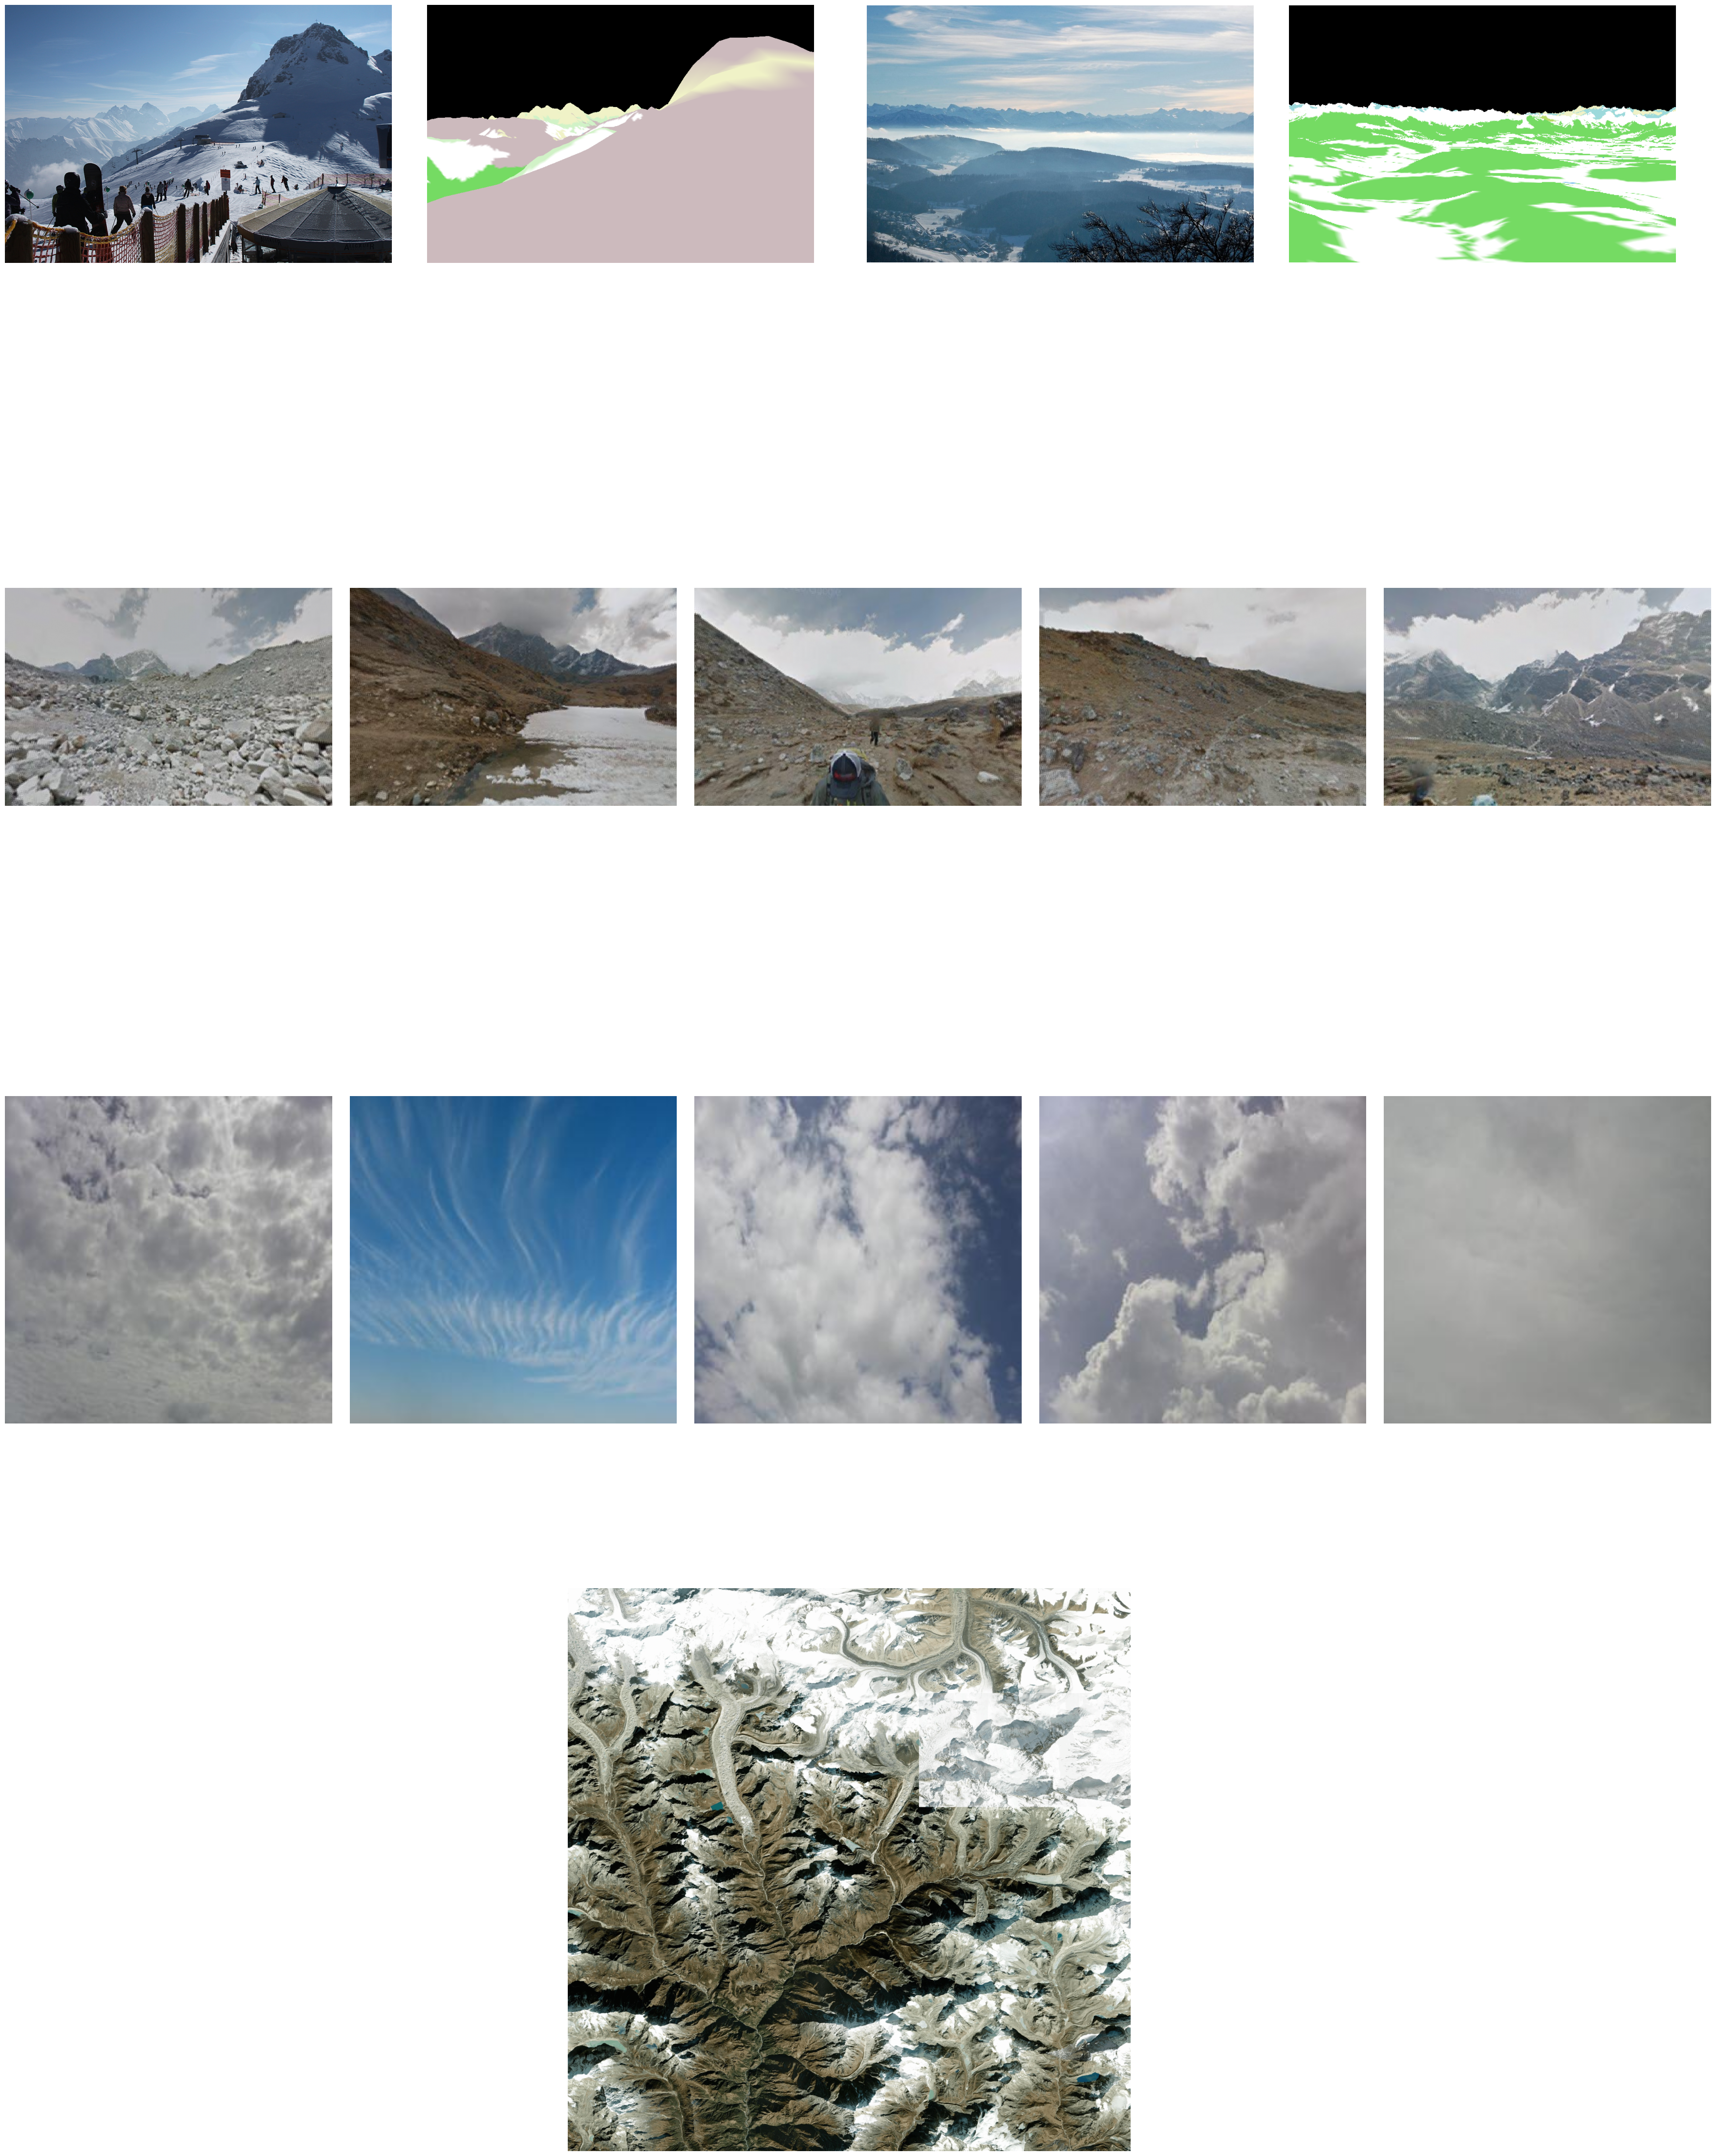
\includegraphics[width=0.92\textwidth]{src/images/figures/fig_dataset_samples.png}
\caption{Sample images from each dataset}
\label{fig:dataset_samples}
\end{figure}


% ============================================================
% APPENDIX F — PLAGIARISM REPORT
% ============================================================
% \chapter{Plagiarism Report}
% \label{app:plagiarism}

% \begin{center}
% \vspace{3cm}
% \fbox{\parbox{0.8\textwidth}{\centering\large
% Attach the plagiarism check report (Turnitin or equivalent) provided by the department here.
% }}
% \vspace{3cm}
% \end{center}
